\scanpage{36}
il y a \deleted{deux pts de} une trajectoire $\Gamma$ fermée de $G$ dans $X$ qui n'est pas contenue dans un ouvert affine. Car on \uline{\unsure{constate}} que l'image inverse de cette trajectoire dans $X\otimes_k\unsure{L|K}=X_{\unsure{K|L}}$ est \deleted{fermée} une \deleted{trajectoire} \inserted{partie} fermée \deleted{\unsure{sous $G$}}, qui n'est contenue dans aucun ouvert affine. \inserted{C'est une trajectoire sous $G\times1$.} De plus, sur cette partie, $1\times G$ opère trivialement, donc les opérations \deleted{du groupe} diagonales de $G$ sont celles de $G\times1$.
\margin{\uline{détailler} \unsure{ce raisonnement} en \uline{lemme}}

\figure{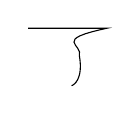
\begin{tikzpicture}\draw (0,0.3)--(1,0.3) .. controls (0.3,0.15) and (0.7,0.1) .. (0.65,-0.05) .. controls (0.7,-0.35) and (0.58,-0.42) .. (0.55,-0.43);\end{tikzpicture}}

\uline{Corollaire} $\underline{\operatorname{Hom}}_{\unsure{L}/K}(\operatorname{Spec}(\unsure{L}),X_{(L)})$ n'existe pas. À fortiori $\underline{\operatorname{Hom}}_K(\operatorname{Spec}(L),X_{(L)})$ n'existe pas.

On fera attention que dans cet exemple,

$K$
% archive foliation: 35
